\chapter{Introduction}\label{ch:introduction}
Personal fabrication devices, such as 3D printers, are already widely used for rapid prototyping and allow non-expert users to create interactive machines, tools and art. As consumer-grade 3D printers are usually desktop-sized, the size of these objects is, however, fairly limited and the creation of large-scale objects is mostly a privilege of industry. TrussFormer aims to enable users to create large-scale dynamic objects using desktop-sized 3D printers. Scale can be achieved by creating multiple small-sized objects and connecting them to each other. Even this technique of breaking down objects into printer-sized parts does not scale, because large models consume material and time proportional to their size. Our solution to this problem is to take ready-made objects, like empty plastic bottles, and only print the connectors that keep them together.\\
To aid users in this process, we developed a software simulation that can create objects which are capable of handling the substantial forces large objects produce. Forces grow cubed with the size of the object, so designing large objects requires substantial engineering skills. We aid users in this process by providing stable primitives which can be attached together. These primitives resemble truss structures - beam-based constructions creating closed triangle surfaces, which are sturdy by design and material-efficient.\\
\begin{figure}[h!]
    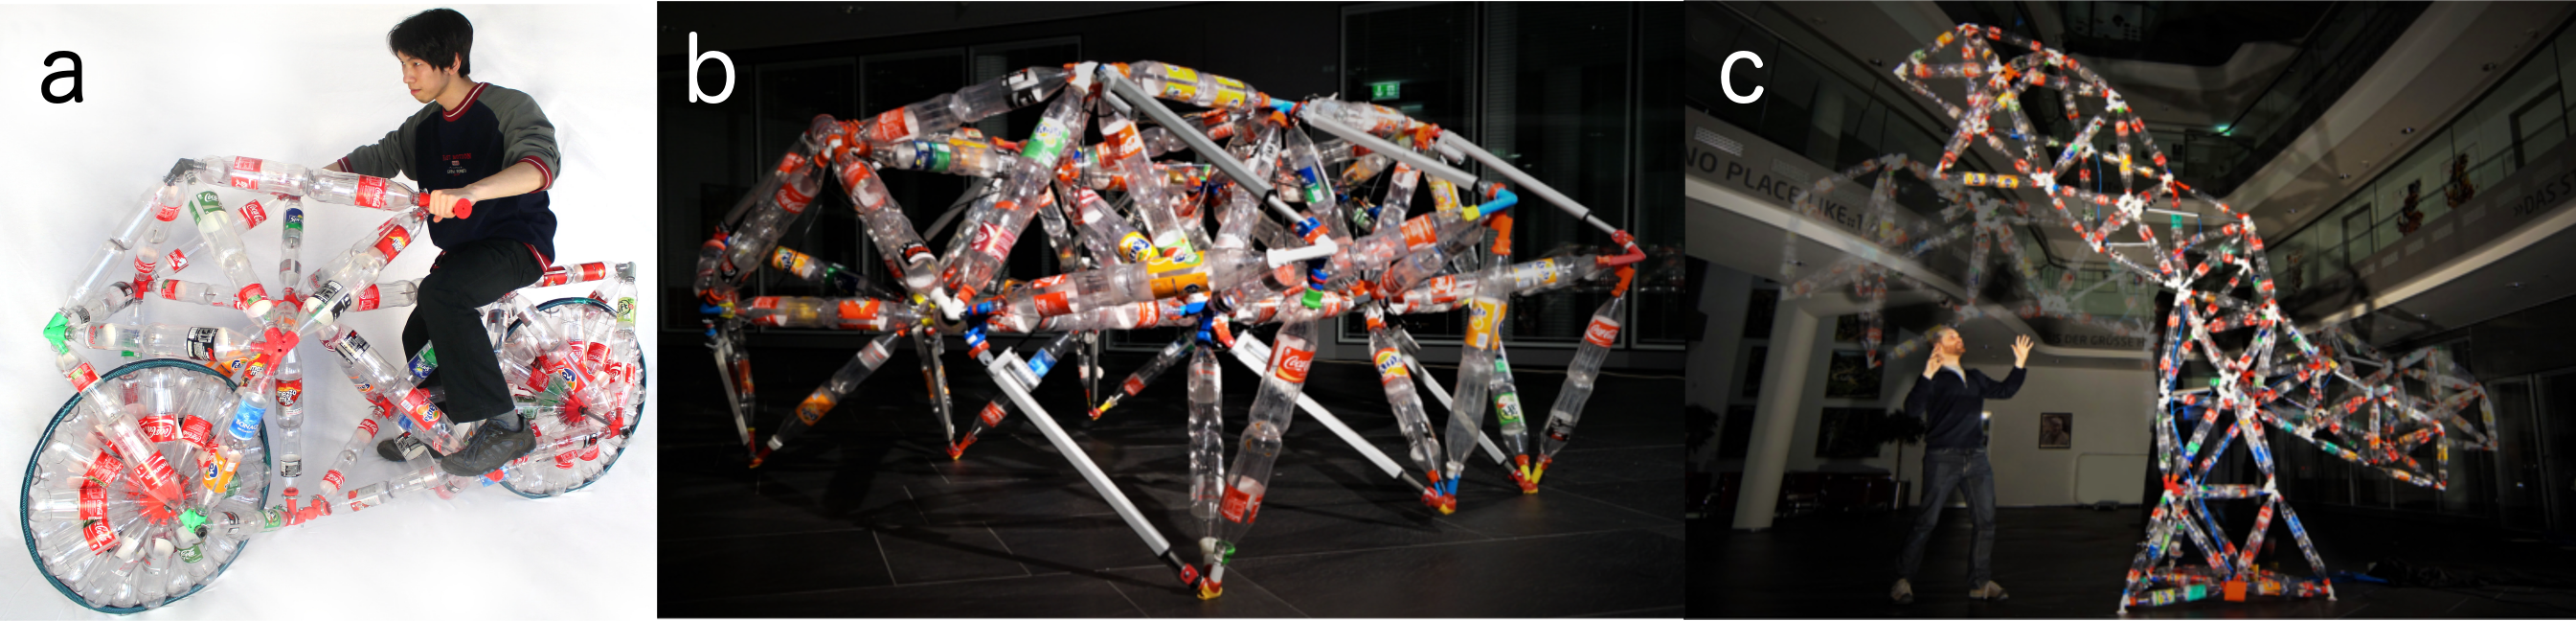
\includegraphics[width=\textwidth]{Introduction/construction_examples.png}
    \centering
    \caption{TrussFormer enables users to create structurally stable truss structures, such as (a) a motor bike, (b) a walking spider robot or (c) an animated T-Rex.}
    \label{fig:examples}
\end{figure}
Such objects have been shown to support a wide range of applications, like furniture or art installation. However, these systems are limited to static structures. Our work is based on \textit{TrussFab} (TODO: Reference TrussFab paper). TrussFab provided possibilities for creating large-scale static truss structures. We want to extend this area of architecture by providing possibilities to create large-scale \textit{kinematic} truss structures. Creating movement in truss structures comes with various challenges. TrussFormer is an end-to-end-system that lets the user create such kinematic structures without needing to have knowledge about the physical properties of moving trusses. It incorporates an editor for virtually creating the desired object, a physics engine that can simulate movement and visualize occurring forces and an export functionality that can convert the created design into 3D printable files.

\section{TrussFormer’s underlying structure achieves stability}
To achieve stability in big structures, TrussFormer incorporates two main ideas. We employ bottles as links in their structurally most sturdy way, i.e. from bottom to bottle neck. As a complement, these links are connected to sturdy ``closed frame structures'', also known as trusses.\\
As demonstrated in Figure \ref{fig:tetra_stability} (a/b), freestanding bottles tend to break easily. Truss structures consist of triangles, which create a structure that prevents deformation, reducing the force on individual bottles. Occurring lateral forces are turned into compression and tension forces along the length of the links. This makes bottles a great choice for trusses. They buckle easily when loaded from the side, but are very strong along their main axis. (c) The resulting structure, such as a tetrahedron, is strong enough to bear the weight of a human. (d) Multiple of these \textit{primitives} can be combined to create truss honeycomb structures. We decided to use tetrahedra and octahedra as primitives, as they are space filling and make construction simpler than, for example, icosahedra.
\begin{figure}[h!]
    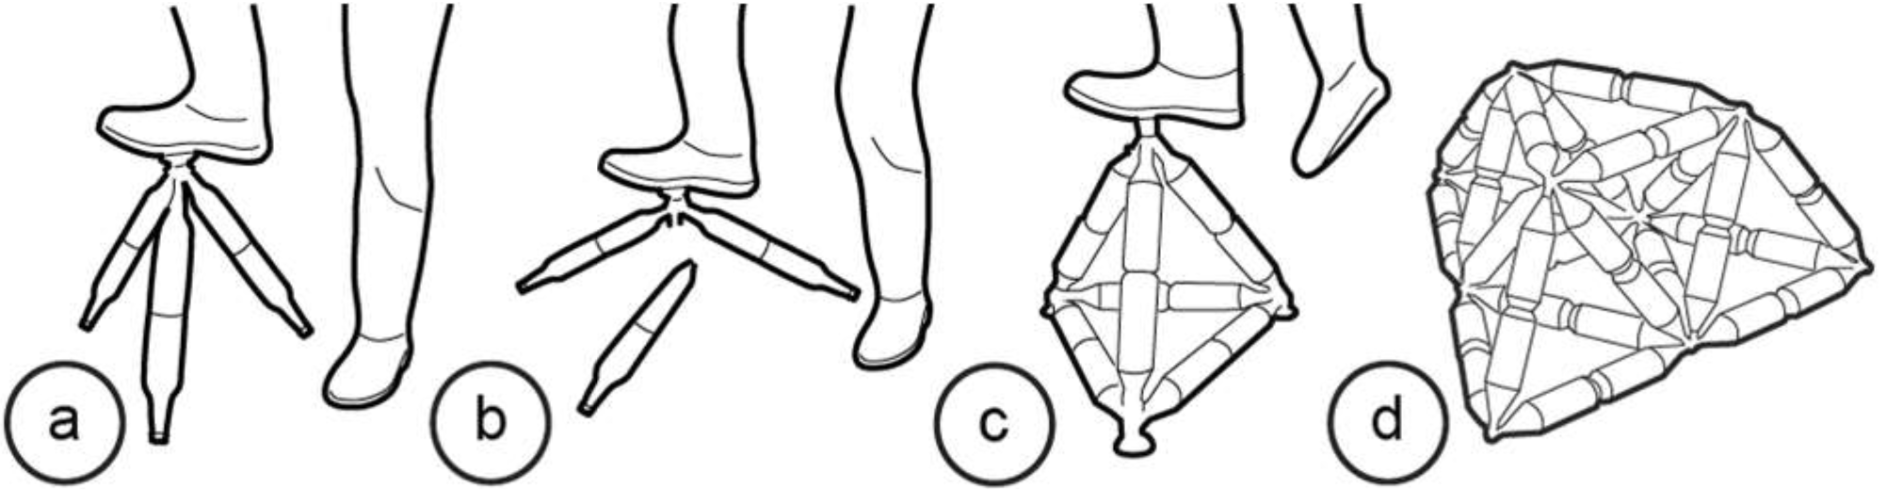
\includegraphics[width=\textwidth]{Introduction/tetra_stability.png}
    \centering
    \caption{(a) Large objects involve large levers, causing them (b) to break under load. (c) TrussFab instead affords structures based on closed triangles, here forming a tetrahedron. Such structures are particularly sturdy. (d) TrussFab extends this concept to tetrahedron-octahedron trusses of arbitrary size.}
    \label{fig:tetra_stability}
\end{figure}

\section{Adding movement using Variable Geometry Trusses}
Apart from creating structurally stable structures, TrussFormer helps users to bring those objects into movement. It does this by incorporating linear actuators into rigid truss structures in a way that they move ``organically'', i.e., hinge around multiple points at the same time. These structures are known as \textit{variable geometry trusses} (TODO: Reference).
Figure \ref{fig:tetra_stability} illustrates this on the smallest elementary truss, (a) the rigid tetrahedron. (b) We swap one of the edges with a linear actuator, (c) resulting in a variable geometry truss. The only required change for this is to introduce hubs that enable rotation at the nodes. We call these hinging hubs.
\begin{figure}[h!]
    \includegraphics[width=\textwidth]{Introduction/moving_tetra_large.png}
    \centering
    \caption{(a) The static tetrahedron (b-c) is converted into a deformable structure by swapping one edge with a linear actuator. The only required change is to introduce connectors that enable rotation.}
    \label{fig:moving_tetra}
\end{figure}
This simple approach to create variable geometry truss mechanisms scales well to arbitrary larger structures. Our T- Rex model from Figure \ref{fig:examples} (c) contains five linear actuators and thus offers five degrees of freedom (DoF). It can (a) lift or lower its neck (1 DoF), (b) turn its head left and right (1 DoF), (c) sweep its tail (2 DoF), and (d) open its mouth (1 DoF), as shown in Figure \ref{fig:t-rex_poses}.
\begin{figure}[h!]
    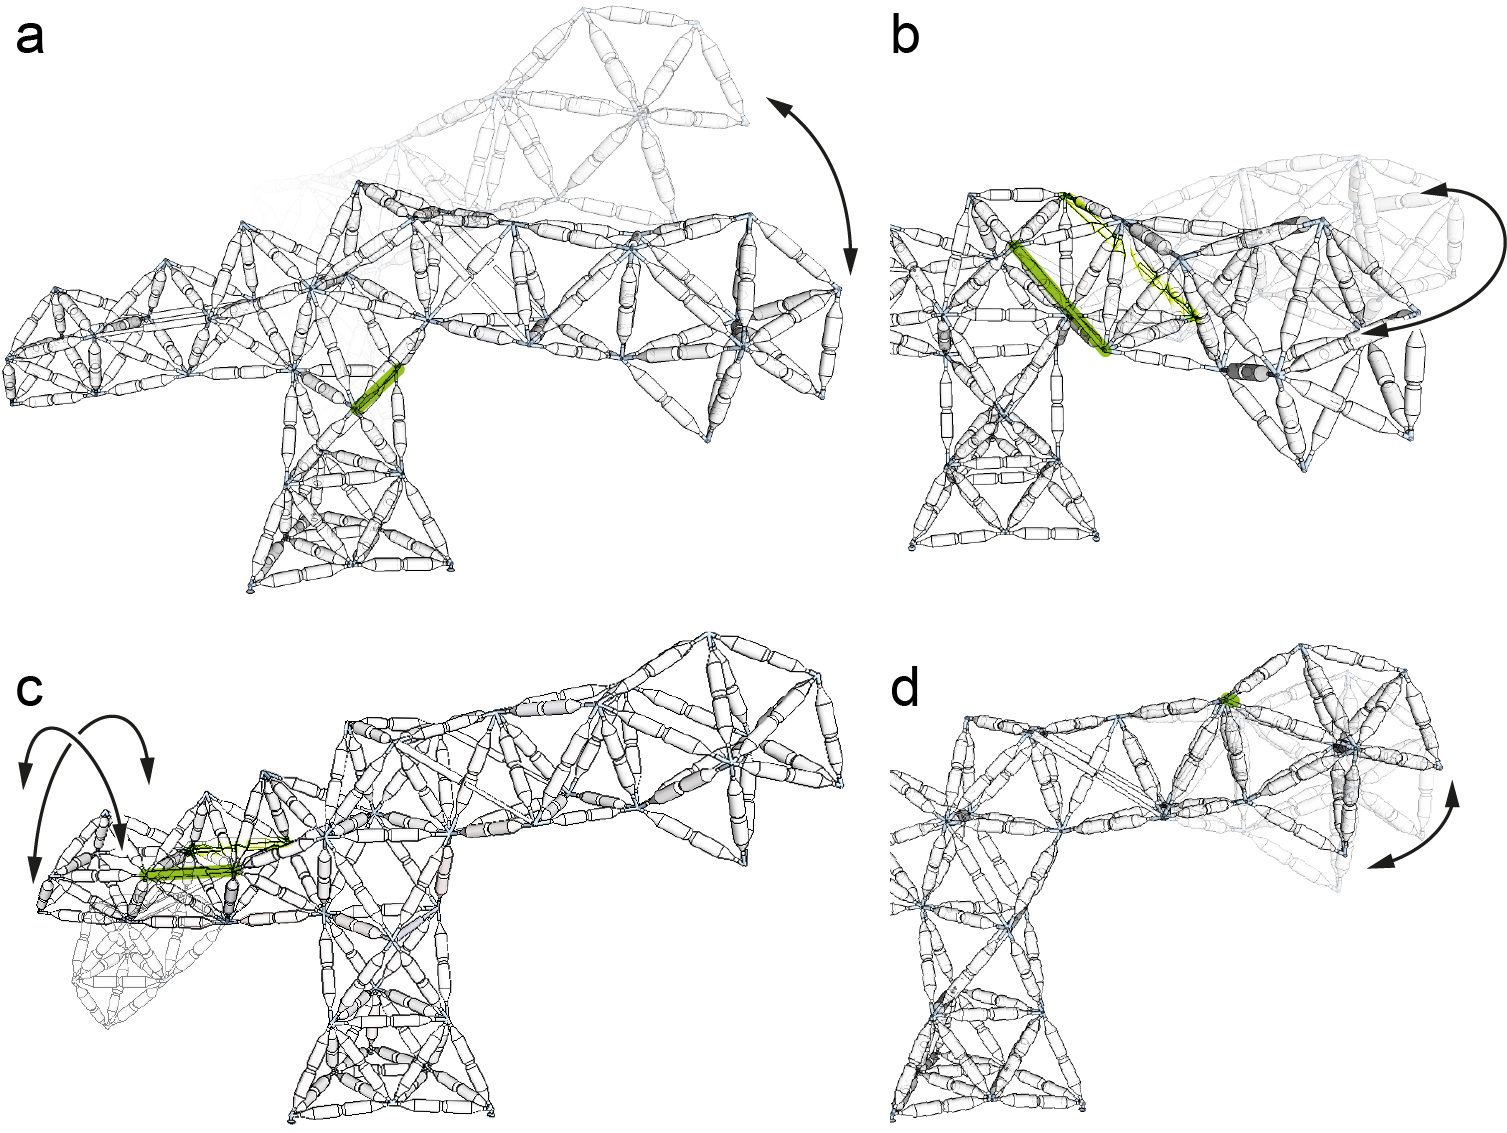
\includegraphics[width=\textwidth]{Introduction/poses_of_the_t-rex.png}
    \centering
    \caption{The T-Rex offers 5 degrees of freedom.}
    \label{fig:t-rex_poses}
\end{figure}

\section{TrussFormer Editor}
The TrussFab editor is the essential part of our system. It is a plugin for the 3D modeling software SketchUp and enables users to create truss structures by placing truss primitives. Apart from designing these truss objects, the editor also allows users to test static and dynamic forces, by displaying then during an interactive simulation, create animations and export the design. Using the export functionality, users can recreate the designed object in the real world by 3D printing the generated STL files and using the exported animation sequence with an Arduino controller.
